\section{Base di dati sistema coordinatore}

\subsection{Abstract}

L'obiettivo è quello di sviluppare un sistema che coordini e decida quando illuminare o non illuminare specifiche zone. Questo sistema dovrà tenere traccia di tutte le informazioni relative allo stato attuale dei lampioni.

Il sistema si collegherà ad altre componenti esterne, utilizzando algoritmi proprietari, e deciderà quando effettuare cambiamenti di stato. Si consiglia la visione del capitolo \ref{cap:sistema-coordinatore}.

%Il riferimento al sistema coordinatore sarà funzionante quando questo documento verrà aggiunto come appendice alla specifica architetturale

\subsection{Analisi dei requisiti}

\subsection{Progettazione concettuale}

\subsection{Progettazione logica}

\subsubsection{Schema concettuale ristrutturato - Schema Logico}

\begin{center}
    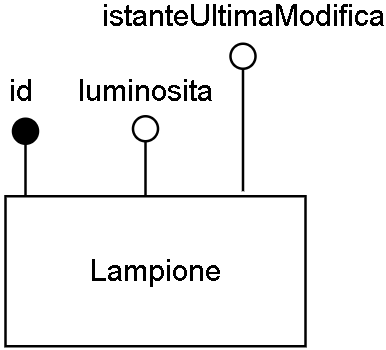
\includegraphics[width=4.5cm]{contenuti/specifica-basi-dati/img-sbd/coordinazione_logico.png}
\end{center}

\subsubsection{Descrizione schema relazionale}

Per questione di compatibilità con il DBMS alcuni nomi di attributi entità e relazioni sono stati normalizzati, utilizzando il camelCase, togliendo gli accenti, accorciando i nomi molto lunghi e con altre piccole accortezze.
La chiave primaria è indicata in \textbf{grassetto}, le chiavi esterne sono indicate con la \underline{sottolineatura}.

\textit{Lampione}(\textbf{id}, luminosita, lastSync)